\documentclass[a4paper, 11pt, twoside]{article}

\usepackage{array}
\usepackage{float}
\usepackage{wrapfig}

% source code
\usepackage{listings}

% set correct hypenation
\usepackage[italian]{babel}

% set margins
\usepackage[
    inner=2.5cm, 
    outer=2.5cm,
    top=3cm,
    bottom=3.75cm
]{geometry}

% set headers
\usepackage{fancyhdr}
\pagestyle{fancyplain}
\fancyhf{}
\setlength{\headheight}{1.3cm}
\rhead{\includegraphics[height=1.25cm]{res/logo_sam}}
\lfoot{SAM 3E - Naoki Pross}
\rfoot{\thepage}

% set font
\usepackage{fontspec}
\setmainfont{Roboto}
\setmonofont{Roboto Mono}

% to fix macros
\usepackage{xspace}
% commands
% macro for project name
\newcommand{\prj}{Z80μPC\xspace}

% invert signal (not, active low)
\newcommand{\inv}[1]{$\overline{\mbox{#1}}$}
 
% metadata
\title{\vspace{-1cm}\texttt{\prj} Single Board \\ Computer Development }
\author{Naoki Pross}

% document 
\begin{document}

\maketitle
\begin{abstract}

    Lo Zilog Z80 \`e un processore a 8 bit che fu introdotto nel 1976 che ebbe
    un grandissimo successo nel mondo dell'elettronica e dell'informatica
    nella fine del 20esimo secolo. In memoria di questo pioniere
    dell'industria dei sistemi informatici questo progetto documenta la
    realizzazione di un microcomputer a scopo generico a base di esso.
    L'obiettivo primario dunque \`e di realizzare una scheda simile ad una
    motherboard dei computers venduti all'epoca completa di RAM, ROMs,
    interfacce seriali e altri circuiti di supporto. Successivamente per
    l'aspetto software il progetto deve implementare i drivers per ogni
    circuito presente sulla scheda in modo da semplificare la programmazione. 
    L'obiettivo secondario del progetto, una volta terminata la costruzione
    hardware, \`e di realizzare una kernel monolitica che offre funzioni
    minimali simili ad un sistema UNIX, quali processi, filesystem, memory
    management e drivers.

\end{abstract}

\section{Specifiche tecniche dello Z80}
Lo Z80 \`e un processore molto minimalistico se paragonato a ci\`o che si
trova oggi sul mercato dei microcontrollori. Per il progetto \prj la CPU in
uso \`e il modello originale \texttt{Zilog Z8400} che non dispone di sistemi
integrati come i modelli SoC odierni. Le specifiche pi\`u importanti sono
elencate a seguire.

\begin{itemize}
    \item Architettura a 8 bit con bus a 16 bit, 64K indirizzi indirizzabili
    \item Registri a 16 bit per {\tt SP,PC} e registri di utilizzo generico a
        8 bit {\tt A..F} combinabili a coppie {\tt AF,BC,..} per utilizzare
        valori a 16 bit
    \item Clock fino a 8 MHz
    \item Segnali di controllo tra cui \texttt{\inv{RD}, \inv{WR},
        \inv{IOREQ}, \inv{MREQ}} e \texttt{\inv{RST}}
    \item Interrupts mascherabili e non con vettore a 8 bit
\end{itemize}

\section{Architettura di base}
Il minimo necessario per far funzionare un computer con lo Z80 sono una ROM e
una RAM, ma per il mio progetto ho scelto di aggiungere dell'hardware
aggiuntivo per lo sviluppo si sistemi pi\`u complessi per apprendere
conoscenze sia nel mondo dell'elettronica che dell'informatica. Per questa 
ragione lo \prj possiede i seguienti componenti:

\begin{center}
\begin{tabular}{ >{\tt}l >{\tt\bfseries}l p{.7\linewidth} }
    % \hline \\
    ROM & M28C64    & EEPROM da 8KB x 8 bit (64K) per il BIOS / Bootloader /
                      OS installata doppia per avere 16KB \\
    RAM & HM62256B  & SRAM da 32KB x 8bit (256K) \\
    CTC & Z8430     & Counter timer circuit ufficiale di Zilog a 4 canali che
                      permette di essere programmato \\
    PIO & Z8420     & Parallel input/output controller di Zilog per avere un
                      intefaccia digitale con due porte da 8 bit \\
    MMU & M4-32/32-15JC & CPLD programmabile che implementa una memory 
                          management unit semplificata in grado di gestire i 5
                          bit pi\`u significativi della linea di indirizzi \\
    USART & TL16C550C & Interfaccia USART per poter comunicare utilizzando il
                        protocollo RS232
\end{tabular}
\end{center}

Oltre a tutto ci\`o per uno scopo formativo lo \prj dispone anche di strumenti
da debug e analisi per comprendere ogni operazione del processore. Il modello
di Z80 scelto \`e in grado di utilizzare un clock fino a 8MHz, ma non
definisce un minimo dunque sono presenti 3 circuiti che generano 3 clock di
velocit\`a differenti.

\begin{center}
\begin{tabular}{ >{\bfseries}r p{.8\linewidth} }
    0Hz     & Questo clock \`e un bottone che permette di creare
              manualmente le pulsazioni del clock, per poter analizzare
              ogni istruzione \\
    200Hz   & Mediante un classico circuito con un LM555 si ha un clock da
              200Hz per eseguire i programmi a velocit\`a rallentata \\
    4MHz    & Clock per esecuzione a velocit\`a piena (normale)
\end{tabular}
\end{center}

Una seconda disposizione per aiutare la comprensione del funzionamento del
processore \`e data da 6 display a 7 segmenti che durante l'esecuzione
rallentata o a step (bottone) visualizzano i bytes presenti sulla bus di
indirizzi a 16 bit e sul bus di dati a 8 bit.

\begin{figure}[!h] \centering
    \includegraphics[width=\linewidth]{res/bus_displays}
    \caption{Display a 7 segmenti per visualizzare il flusso di dati della
    CPU}
\end{figure}

\section{Memory Management Unit}

Alcuni modelli successori dello Z8400 implementavano una MMU SoC che
permetteva di indirizzare un address space di dimensione maggiore. Per lo \prj
non necessito di un indirizzamento pi\`u grande ma piuttosto sono interessato
dalle operazioni di gestione della memoria di una MMU simile a ci\`o che
accade nelle architetture X86. Nelle architetture odierne basate sull'X86/64
\`e presente un sistema di traslazione di indirizzi di memoria da virtuale a
fisica. Con lo scopo di trarne solamente i vantaggi pi\`u fondamentali lo \prj
implementa nella CPLD MMU un sistema basilare di gestione di pagine di memoria
con traslazione di indirizzi in modo da poter allocare pi\`u programmi nella
RAM anche se il sistema non implementa il multitasking.

% TODO: write about this in more details

\subsection{Address Space}

\begin{wrapfigure}{r}{.4\linewidth} \centering
    \vspace{8mm}
    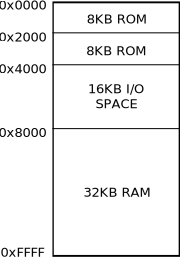
\includegraphics[width=.9\linewidth]{res/addrspace}
    \vspace{4mm}
    \caption{Address space dello \prj}
\end{wrapfigure}
La funzione primaria della MMU \`e di mappare i dispositivi I/O e le memorie
nell'address space. Nell'implementazione reale la MMU controlla i segnali {\tt
\inv{CS}} seguendo una logica combinatoria molto semplice che controlla se
l'indirizzo sul bus si trova in una zona definita per un dispositivo.
L'address space si presenta dunque nella seguente maniera, per cui la ROM
occupa il primo quarto, i dispositivi mappabili il secondo quarto e la RAM la
met\`a restante. Essendo un progetto pensato per essere esteso 16KB sono
liberi per mappare dispositivi esterni collegati attraverso il connettore 
DIN41612.

% \begin{wrapfigure}{l}{.4\linewidth} \centering
%     \includegraphics[width=.8\linewidth]{res/iospace}
% \end{wrapfigure}

\subsection{Page Table}

Per poter controllare la traslazione degli indirizzi la MMU dispone di una
Page Table a cui \`e possibile accedere attraversso un certo indirizzo
nell'I/O space. La page table di 5 bit permette la gestione delle regioni di
memoria da impostare per dei determinati processi. Questa funzione \`e 
importante perch\`e permette la separazione dello stack e della memoria della
kernel dai programmi normali. Per lo \prj potrebbe sembrare eccessivo ma
essendo uno strumento per apprendere le fondamenta dell'elettronica e
dell'informatica \`e interessante implementare questa funzionalit\`a che
comunque se necessario pu\`o essere disabilitata.

\section{Schema a blocchi}

\begin{figure}[!h] \centering
    \includegraphics[width=.85\linewidth]{res/block_diagram}
\end{figure}

\section{Software / Sistema operativo}

Negli sviluppi pi\`u recenti intorno allo Z80 esso veniva utilizzato come un
microcontrollore anzich\`e come processore da computer, per questa ragione non
sono presenti molti sistemi operativi per questa piattaforma. Dunque per lo
\prj il progetti implementa un sistema operativo soprannominato {\tt
HelvetiOS} con le funzioni minime necessarie come un interfaccia seriale a
comandi e un meccanismo per caricare i programmi.

\subsection{Componenti di base}

Per garantire un funzionamento minimo il sistema {\tt HelvetiOS} deve offrire
drivers e utility di base quali:

\begin{center}
\begin{minipage}[t]{.4\linewidth}
    \begin{itemize}
        \item USART driver and API
        \item PIO driver and API
        \item CTC driver and API
    \end{itemize}
\end{minipage}%
\begin{minipage}[t]{.4\linewidth}
    \begin{itemize}
        \item Bootloader
        \item Program launcher
        \item Shell-like interface
    \end{itemize}
\end{minipage}
\end{center}

\subsection{Interfacce dell'API} 

Nel corso dello sviluppo questa sezione verr\`a continuamente espansa per
documentare le interfacce dei vari drivers.

\subsubsection{USART}
\begin{lstlisting}[language=C, basicstyle=\ttfamily]
void usart_set_baudrate(uint16_t baudrate);
void usart_set_parity(int mode);
void usart_set_stop_bits(int count);
void usart_set_word_length(int length);
void usart_set_autoflow(int mode);

inline void usart_init(uint16_t baudrate, int parity, int stop_bits); 

void usart_transmit(uint8_t data);
uint8_t usart_receive();

int usart_write(uint8_t *data, size_t size);
int usart_read(uint8_t *buffer, size_t count);
\end{lstlisting}

% \subsection{PIO}

\subsection{Toolchain per la compilazione}

Per compilare il software del progetto si utilizza SDCC, un progetto
open-source che supporta la compilazione di binari per l'architettura dello
Z80. Nella mia configurazione utilizzo GNU make con il seguente makefile.

\newpage
\begin{lstlisting}[language=make, numbers=left, basicstyle=\ttfamily]
####
# Source code settings
#
OSNAME := helvetiOS

CSOURCES    := $(wildcard kernel/*.c) $(wildcard libc/*.c)
OBJECTS     := $(patsubst %.c,build/%.rel,$(CSOURCES))
HEXFILE     := build/$(OSNAME).hex
BINARY      := build/$(OSNAME).bin

###
# Compiler settings

CC      := sdcc

CFLAGS  := -mz80 \
            -I kernel/include -I libc/include -DDEBUG

LDFLAGS := -mz80 --no-std-crt0 crt0.rel \
            --code-loc 0x0800 --data-loc 0x8000

.PHONY: dirs dis clean
all: $(BINARY)

# build binary
$(BINARY): $(OBJECTS) dirs
    $(CC) $(LDFLAGS) $(OBJECTS) -o $(HEXFILE)
    xxd -r -p $(HEXFILE) $(BINARY)

$(OBJECTS): build/%.rel : %.c $(CSOURCES) dirs crt0.rel
    $(CC) $(CFLAGS) -c $< -o $@

crt0.rel: crt0.s
    sdasz80 -o $<

dirs:
    mkdir -p build build/kernel build/libc

dis: $(BINARY)
    z80dasm -a -g 0h $< -o $(OSNAME).s

clean:
    - rm -rd build/*
    - rm $(OSNAME).s
    - rm crt0.rel
\end{lstlisting}

\end{document}
